% Generazione delle variabili che andranno a sostituire quelle del template `HomePage.tex`
\newcommand{\documento}{\SdF}
\newcommand{\nomedocumentofisico}{StudioDiFattibilit\`a\_v1\_0\_0.pdf}
\newcommand{\redazione}{\LC\\ & \TG\\ & \CV\\ & \SG\\ & \NC\\ & \MM}
\newcommand{\verifica}{\LC\\ & \TG}
\newcommand{\approvazione}{\CV}
\newcommand{\uso}{Interno}
\newcommand{\destinateTo}{\TV, \\ & \RC, \\ & \II}

\newcommand{\datacreazione}{22 novembre 2018}
\newcommand{\datamodifica}{07 Gennaio 2016}
\newcommand{\stato}{Approvato}

\def\TABELLE{false}	% abilita - disabilita l'indice delle tabelle
\def\FIGURE{false} 	% abilita - disabilita l'indice delle figure

% Layout del documento 
\documentclass[a4paper,11pt]{article}

\usepackage{ifthen}
\usepackage[english,italian]{babel}
\usepackage[utf8]{inputenc}
\usepackage[T1]{fontenc}
\usepackage{float}
\usepackage{chapterbib}
\usepackage{graphicx}
\usepackage[a4paper,top=2.5cm,bottom=2.5cm,left=2.5cm,right=2.5cm]{geometry}

\PassOptionsToPackage{hyphens}{url}\usepackage[hyperfootnotes=false]{hyperref}
\hypersetup{%
	colorlinks=true,
	citecolor=black,
	linkcolor=black,
	urlcolor=blue
}

\usepackage{enumitem}
\usepackage{eurosym}
\usepackage{booktabs}
\usepackage{fancyhdr}
\usepackage{totpages}
\usepackage{tabularx, array}
\usepackage{dcolumn}
\usepackage{epstopdf}
\usepackage{booktabs}
\usepackage{fancyhdr}
\usepackage{longtable}
\usepackage{calc}
\usepackage{datatool}
\usepackage[bottom]{footmisc}
\usepackage{listings}
\usepackage{textcomp}
\usepackage{titlesec}
\usepackage{rotating}
\usepackage{multirow}
\usepackage{placeins}
\usepackage{color}
\usepackage{makecell}
\usepackage{lscape}
 
\usepackage[table,usenames,dvipsnames]{xcolor}
% Definizione di nuovi colori da poter usare per le tabelle
\definecolor{lightgray}{gray}{0.92}
\definecolor{lightblue}{rgb}{0.93,0.95,1.0}
\definecolor{headgray}{gray}{0.88}

% Ridefinizione dell'env tabularx. Il vecchio è utilizzabile con l'env oldtabularx
\let\oldtabularx\tabularx
\let\endoldtabularx\endtabularx
\renewenvironment{tabularx}{\rowcolors{2}{white}{lightgray}\oldtabularx}{\endoldtabularx}

% Per tabularx con padding, parametro tra [], eg [1.3]
\newenvironment{paddedtablex}[1][1]{%
	\renewcommand*{\arraystretch}{#1}%
	\renewcommand\theadfont{\bfseries}%
	\tabularx%
}{%
	\endtabularx
}

% Ridefinizione dell'env tabular. Il vecchio è utilizzabile con l'env oldtabular
\let\oldtabular\tabular
\let\endoldtabular\endtabular
\renewenvironment{tabular}{\rowcolors{2}{lightgray}{white}\oldtabular}{\endoldtabular}

% Per tabular con padding, parametro tra [], eg [1.3]
\newenvironment{paddedtable}[1][1]{%
	\renewcommand*{\arraystretch}{#1}%
	\renewcommand\theadfont{\bfseries}%
	\tabular%
}{%
	\endtabular
}

% ***TABELLA ANALISI RISCHI PDP***

\newenvironment{risktable}[1][1]{%
	\centering%
	\renewcommand*{\arraystretch}{1.4}%
	\renewcommand\theadfont{\bfseries}%
	\oldtabularx%
}{%
	\endoldtabularx
}

% ***TABELLA SUDDIVISIONE DEL LAVORO PDP***

\newenvironment{detailtable}[1][1]{%
	\centering%
	\renewcommand*{\arraystretch}{1.4}%
	\renewcommand\theadfont{\bfseries}%
	\oldtabularx%
}{%
	\endoldtabularx
}

% ***TABELLA ORGANIGRAMMA***

\newenvironment{orgtable}[1][1]{%
	\centering%
	\renewcommand*{\arraystretch}{1.4}%
	\renewcommand\theadfont{\bfseries}%
	\oldtabularx%
}{%
	\endoldtabularx
}


% DA SPOSTARE SU COMANDI
% ***DOUBLE LINE***

\def\mydoublerule#1#2#3{%%
	\hrule width#1 height#2 \vskip#2
	\hrule width#1 height#3 
}

% ***NUOVO TIPO DI CELLA CENTRATA***

\newcolumntype{Y}{>{\centering\arraybackslash}X}

% ***STILE PAGINA***
\pagestyle{fancy}

% ***INTESTAZIONE***
\rhead{\Large{\progetto} \\ \footnotesize{\documento}}
\lhead{
\includegraphics[keepaspectratio = true, width = 25px]{../template/icons/a6(1).png}}

% ***PIÈ DI PAGINA***
\lfoot{\textit{\gruppo} \\
\footnotesize{\email}}

\rfoot{\thepage} % per le prime pagine: mostra solo il numero romano
\cfoot{}
\renewcommand{\footrulewidth}{0.4pt}   % Linea sopra il piè di pagina
\renewcommand{\headrulewidth}{0.4pt}  % Linea sotto l'intestazione

% ***INSERIMENTO DI NUOVE SOTTOSEZIONI
\setcounter{secnumdepth}{7} %mostra nel documento fino al livello 8 (1.2.3.4.5.6.7.8)
\setcounter{tocdepth}{7}    % mostra nell'indice fino al livello 8 (1.2.3.4.5.6.7.8)


\makeatletter
\newcounter{subsubparagraph}[subparagraph]
\renewcommand\thesubsubparagraph{%
	\thesubparagraph.\@arabic\c@subsubparagraph}
\newcommand\subsubparagraph{%
	\@startsection{subsubparagraph}    % counter
	{6}                              % level
	{\parindent}                     % indent
	{3.25ex \@plus 1ex \@minus .2ex} % beforeskip
	{0.75em}                           % afterskip
	{\normalfont\normalsize\bfseries}}
\newcommand\l@subsubparagraph{\@dottedtocline{6}{10em}{5.5em}} %gestione dell'indice
\newcommand{\subsubparagraphmark}[1]{}
\makeatother

\makeatletter
\newcounter{subsubsubparagraph}[subsubparagraph]
\renewcommand\thesubsubsubparagraph{%
	\thesubsubparagraph.\@arabic\c@subsubsubparagraph}
\newcommand\subsubsubparagraph{%
	\@startsection{subsubsubparagraph}    % counter
	{7}                              % level
	{\parindent}                     % indent
	{3.25ex \@plus 1ex \@minus .2ex} % beforeskip
	{0.75em}                           % afterskip
	{\normalfont\normalsize\bfseries}}
\newcommand\l@subsubsubparagraph{\@dottedtocline{7}{10em}{6.5em}} %gestione dell'indice
\newcommand{\subsubsubparagraphmark}[1]{}
\makeatother


\addtocounter{vZ}{1}
\newcommand{\modifiche}
{
	% \addToDiary{Inserimento qualità di processo}{\Ver}{\NC}{03-01-2018}
	% \addToDiary{Inserimento qualità di prodotto}{\Ver}{\NC}{30-12-2018}
	% \addToDiary{Inserimento standard ISO 90003}{\Ver}{\NC}{27-12-2018}
	% \addToDiary{Inserimento standard ISO 9126}{\Ver}{\NC}{26-12-2018}
	% \addToDiary{Inserimento standard ISO 15504}{\Ver}{\NC}{23-12-2018}
	
	\addToDiary{Aggiunto appendice \S{C} (mitigazione variazioni)}{\Ver}{\MM}{14-02-2019}

	% 1.Y.Z
	\setcounter{vX}{1}%
	\setcounter{vY}{0}%
	\setcounter{vZ}{0}%

	\addToDiary{Approvazione per il rilascio}{\Res}{\NC}{13-01-2019}

	% 0.2.Z
	\decrvX
	\setcounter{vY}{2}%
	\setcounter{vZ}{0}%

	\addToDiary{Verifica finale}{\Ver}{\MM}{12-01-2019}

    % 0.1.Z
    \decrvY%
	\setcounter{vZ}{2}%

	\addToDiary{Aggiunto appendice ``Valutazioni per il miglioramento''}{\Ver}{\MM}{11-01-2019}
	\addToDiary{Inserito ``Resoconto delle attività di verifica''}{\Ver}{\NC}{08-01-2019}
	\addToDiary{Verifica documento}{\Ver}{\CV}{10-12-2018}

    % 0.0.Z
	\setcounter{vZ}{5}%
	\decrvY%

	\addToDiary{Aggiunto appendice ``Standard di qualità''}{\Ver}{\NC}{03-12-2018}
	\addToDiary{Inserito ``Qualità di processo''}{\Ver}{\NC}{02-12-2018}
	\addToDiary{Inserito ``Qualità di prodotto''}{\Ver}{\TG}{01-12-2018}
	\addToDiary{Aggiunta Introduzione}{\Ver}{\NC}{29-11-2018}
    \addToDiary{Creazione template}{\Red}{\TG}{27-11-2018}
}


% Comandi generali
% Generali
\newcommand{\progetto}{Butterfly}
\newcommand{\gruppo}{AlphaSix}
\newcommand{\email}{alpha.six.unipd@gmail.com}

% Documenti
\newcommand{\AdR}{Analisi dei Requisiti}
\newcommand{\NdP}{Norme di Progetto}
\newcommand{\PdP}{Piano di Progetto}
\newcommand{\SdF}{Studio di Fattibilità}
\newcommand{\PdQ}{Piano di Qualifica}
\newcommand{\VI}{Verbale Interno}
\newcommand{\VE}{Verbale Esterno}
\newcommand{\ST}{Specifica Tecnica}
\newcommand{\DDP}{Definizione di Prodotto}
\newcommand{\MU}{Manuale Utente}
\newcommand{\Gl}{Glossario}
\newcommand{\LdP}{Lettera di Presentazione}
\newcommand{\AdRv}{AnalisiDeiRequisiti v2.0.0}
\newcommand{\NdPv}{NormeDiProgetto v2.0.0}
\newcommand{\PdPv}{PianoDiProgetto v2.0.0}
\newcommand{\PdQv}{PianoDiQualifica v2.0.0}
\newcommand{\SdFv}{StudioDiFattibilità v1.0.0}
\newcommand{\DdPv}{DefinizioneDiprodotto v1.0.0}
\newcommand{\Glv}{Glossario v2.0.0}

% Componenti del gruppo
\newcommand{\LC}{Laura Cameran}
\newcommand{\TG}{Timoty Granziero}
\newcommand{\CV}{Ciprian Voinea}
\newcommand{\SG}{Samuele Gardin}
\newcommand{\NC}{Nicola Carlesso}
\newcommand{\MM}{Matteo Marchiori}

% Ruoli
\newcommand{\RdP}{Responsabile di Progetto}
\newcommand{\Res}{Responsabile}
\newcommand{\Red}{Redattore}
\newcommand{\Amm}{Amministratore}
\newcommand{\Ver}{Verificatore}
\newcommand{\Prog}{Progettista}
\newcommand{\Progr}{Programmatore}
\newcommand{\Ana}{Analista}
\newcommand{\RdPs}{Responsabili di Progetto}
\newcommand{\Ress}{Responsabile}
\newcommand{\Amms}{Amministratori}
\newcommand{\Vers}{Verificatori}
\newcommand{\Progs}{Progettisti}
\newcommand{\Progrs}{Programmatori}
\newcommand{\Anas}{Analisti}

% Professori e proponente
\newcommand{\TV}{Prof. Tullio Vardanega}
\newcommand{\RC}{Prof. Riccardo Cardin}
\newcommand{\LuC}{Luca Cappelletti}
\newcommand{\DZ}{Davide Zanetti}
\newcommand{\II}{Imola Informatica}
\newcommand{\proponente}{Imola Informatica}

% Comando per una nuova riga nella tabella del diario delle modifiche
\newcommand{\specialcell}[2][c]{%
	\begin{tabular}[#1]{@{}c@{}}#2\end{tabular}}

\renewcommand*\sectionmark[1]{\markboth{#1}{}}
\renewcommand*\subsectionmark[1]{\markright{#1}}

% Pediodi di lavoro 
\newcommand{\AR}{Analisi dei Requisiti}
\newcommand{\AD}{Analisi dei Requisiti in Dettaglio}
\newcommand{\PA}{Progettazione Architetturale}
\newcommand{\PD}{Progettazione di Dettaglio}
\newcommand{\CO}{Codifica}
\newcommand{\VV}{Validazione}

% Revisioni
\newcommand{\RR}{Revisione dei Requisiti}
\newcommand{\RP}{Revisione di Progettazione}
\newcommand{\RQ}{Revisione di Qualifica}
\newcommand{\RA}{Revisione di Accettazione}

\newcommand{\myincludegraphics}[2][]{%
	\setbox0=\hbox{\phantom{X}}%
	\vtop{
		\hbox{\phantom{X}}
		\vskip-\ht0
		\hbox{\includegraphics[#1]{#2}}}}

% Ridefinizione linea per le note a piè di pagina
\renewcommand{\footnoterule}{%
  \kern -3pt
  \hrule width \textwidth height 0.4pt
  \kern 2pt
}

\colorlet{punct}{red!60!black}
\definecolor{background}{HTML}{EEEEEE}
\definecolor{delim}{RGB}{20,105,176}
\colorlet{numb}{magenta!60!black}
\lstdefinelanguage{json}{
 	basicstyle=\small\ttfamily,
 	numbers=left,
 	numberstyle=\scriptsize,
 	stepnumber=1,
 	numbersep=8pt,
 	showstringspaces=false,
 	breaklines=true,
 	frame=lines,
 	backgroundcolor=\color{background},
 	literate=
 	*{0}{{{\color{numb}0}}}{1}
 	{1}{{{\color{numb}1}}}{1}
 	{2}{{{\color{numb}2}}}{1}
 	{3}{{{\color{numb}3}}}{1}
 	{4}{{{\color{numb}4}}}{1}
 	{5}{{{\color{numb}5}}}{1}
 	{6}{{{\color{numb}6}}}{1}
 	{7}{{{\color{numb}7}}}{1}
 	{8}{{{\color{numb}8}}}{1}
 	{9}{{{\color{numb}9}}}{1}
 	{:}{{{\color{punct}{:}}}}{1}
 	{,}{{{\color{punct}{,}}}}{1}
 	{\{}{{{\color{delim}{\{}}}}{1}
 	{\}}{{{\color{delim}{\}}}}}{1}
 	{[}{{{\color{delim}{[}}}}{1}
 	{]}{{{\color{delim}{]}}}}{1},
}
\lstset{language=json}
\lstset{literate=%
    {Ö}{{\"O}}1
 	{Ä}{{\"A}}1
 	{Ü}{{\"U}}1
 	{é}{{\"s}}1
 	{è}{{\"e}}1
 	{à}{{\"a}}1
	{ö}{{\"o}}1
}


\definecolor{listinggray}{gray}{0.9}
\definecolor{lbcolor}{rgb}{0.9,0.9,0.9}

\lstset{
  backgroundcolor=\color{lbcolor},
  tabsize=4,
  language=Python,
  captionpos=b,
  frame=single,
  numbers=left,
  numberstyle=\tiny,
  numbersep=5pt,
  breaklines=true,
  showstringspaces=false,
  basicstyle=\footnotesize,
  % identifierstyle=\color{magenta},
  keywordstyle=\bfseries\color[rgb]{0,0,1},
  commentstyle=\color[rgb]{0,0.6,0},
  stringstyle=\color{red}
}

% \definecolor{mygreen}{rgb}{0,0.6,0}
% \definecolor{mygray}{rgb}{0.5,0.5,0.5}
% \definecolor{mymauve}{rgb}{0.58,0,0.82}

% \lstset{ 
%   backgroundcolor=\color{white},   % choose the background color; you must add \usepackage{color} or \usepackage{xcolor}; should come as last argument
%   basicstyle=\footnotesize,        % the size of the fonts that are used for the code
%   breakatwhitespace=false,         % sets if automatic breaks should only happen at whitespace
%   breaklines=true,                 % sets automatic line breaking
%   captionpos=b,                    % sets the caption-position to bottom
%   commentstyle=\color{mygreen},    % comment style
%   deletekeywords={...},            % if you want to delete keywords from the given language
%   escapeinside={\%*}{*)},          % if you want to add LaTeX within your code
%   extendedchars=true,              % lets you use non-ASCII characters; for 8-bits encodings only, does not work with UTF-8
%   firstnumber=1000,                % start line enumeration with line 1000
%   frame=single,	                   % adds a frame around the code
%   keepspaces=true,                 % keeps spaces in text, useful for keeping indentation of code (possibly needs columns=flexible)
%   keywordstyle=\color{blue},       % keyword style
%   language=Octave,                 % the language of the code
%   morekeywords={*,...},            % if you want to add more keywords to the set
%   numbers=left,                    % where to put the line-numbers; possible values are (none, left, right)
%   numbersep=5pt,                   % how far the line-numbers are from the code
%   numberstyle=\tiny\color{mygray}, % the style that is used for the line-numbers
%   rulecolor=\color{black},         % if not set, the frame-color may be changed on line-breaks within not-black text (e.g. comments (green here))
%   showspaces=false,                % show spaces everywhere adding particular underscores; it overrides 'showstringspaces'
%   showstringspaces=false,          % underline spaces within strings only
%   showtabs=false,                  % show tabs within strings adding particular underscores
%   stepnumber=2,                    % the step between two line-numbers. If it's 1, each line will be numbered
%   stringstyle=\color{mymauve},     % string literal style
%   tabsize=2,	                   % sets default tabsize to 2 spaces
%   title=\lstname                   % show the filename of files included with \lstinputlisting; also try caption instead of title
% }

\newcommand{\impl}{\textcolor{Green}{Implementato}}
\newcommand{\implno}{\textcolor{Red}{Non Implementato}}

% G di glossario a pedice, con e senza spazio
\newcommand{\GAlt}{\ped{\tiny{G}}}
\newcommand{\G}{\ped{\tiny{G }}}

% e.g. \gloss{progetto}
\newcommand{\gloss}[1]{%
    {\small \textsc{#1}}\GAlt%
}

% D di documento a pedice, con e senza spazio
% \newcommand{\DAlt}{\ped{\tiny{D}}}
\newcommand{\D}{\ped{\tiny{D}}}

% e.g. \Doc{Norme di Progetto}
\newcommand{\Doc}[1]{\textit{#1}\D}

% Comandi per applicare \Doc con un comando unico
\newcommand{\PdQd}{\Doc{\PdQv}}
\newcommand{\PdPd}{\Doc{\PdPv}}
\newcommand{\NdPd}{\Doc{\NdPv}}
\newcommand{\AdRd}{\Doc{\AdRv}}
\newcommand{\SdFd}{\Doc{\SdFv}}
\newcommand{\Gld}{\Doc{\Gld}}

% Le sottosezioni paragraph, subparagraph ecc.. vengono visualizzate come section
\titleformat{\paragraph}{\normalfont\normalsize\bfseries}{\theparagraph}{1em}{}
\titlespacing*{\paragraph}{0pt}{3.25ex plus 1ex minus .2ex}{1.5ex plus .2ex}

\titleformat{\subparagraph}{\normalfont\normalsize\bfseries}{\thesubparagraph}{1em}{}
\titlespacing*{\subparagraph}{0pt}{3.25ex plus 1ex minus .2ex}{1.5ex plus .2ex}

\titleformat{\subsubparagraph}{\normalfont\normalsize\bfseries}{\thesubsubparagraph}{1em}{}
\titlespacing*{\subsubparagraph}{0pt}{3.25ex plus 1ex minus .2ex}{1.5ex plus .2ex}

\titleformat{\subsubsubparagraph}{\normalfont\normalsize\bfseries}{\thesubsubsubparagraph}{1em}{}
\titlespacing*{\subsubsubparagraph}{0pt}{3.25ex plus 1ex minus .2ex}{1.5ex plus .2ex}


% Indentazione paragrafi rimossa. Per metterla manualmente, precedere il paragrafo con il comando /indent
\newlength\tindent
\setlength{\tindent}{\parindent}
\setlength{\parindent}{0pt}
\renewcommand{\indent}{\hspace*{\tindent}}


% Generazione automatica dei numeri per le versioni
\newcounter{vX} % valore per X in X.Y.Z
\newcounter{vY} % valore per Y in X.Y.Z
\newcounter{vZ} % valore per Z in X.Y.Z
\newcommand{\decrvX}{\addtocounter{vX}{-1}} % Comando per il decremento automatico del counter vZ
\newcommand{\decrvY}{\addtocounter{vY}{-1}} % Comando per decrementare vY
\newcommand{\decrvZ}{\addtocounter{vZ}{-1}} % Comando per decrementare vZ
\newcommand{\addToDiary}[4]{\thevX.\thevY.\thevZ & #1 & #2 & #3 & #4\decrvZ\\} % Comando per generare una riga di diario delle modifiche (\addToDiary{desc}{ruolo}{nominativo}{data})

% Colore righe grigie
\newcommand{\tablegray}{gray!20}

% Stile liste
% \renewcommand\labelitemi{$\circ$} % Bullet, primo livello
% \renewcommand\labelitemii{$\diamond$} % Bullet, primo livello
% \renewcommand\labelitemii{\normalfont\bfseries \textendash} % --, secondo livello
% \renewcommand\labelitemiii{\textasteriskcentered} % *, terzo livello
% \renewcommand\labelitemiv{\textperiodcentered} % ., quarto livello
% \setlist[itemize,2]{label=$\circ$}
% \setlist[itemize,2]{label=$\diamond$}

% Placeholder sui diari
\newcommand{\pl}{Placeholder}

%Comandi per le versioni delle tecnologie
\newcommand{\python}{Python 3.6.7}
\newcommand{\gitlab}{GitLab 11.7}
\newcommand{\redmine}{Redmine 4.0.1}
\newcommand{\kafka}{Apache Kafka 2.12}
\newcommand{\docker}{Docker 18.09}
\newcommand{\telegram}{Telegram (Bot API 4.0)}
\newcommand{\slack}{Slack}
\newcommand{\jenkins}{Jenkins 2.146}



\setcounter{secnumdepth}{4}
\setcounter{tocdepth}{4}

\begin{document}
	
	% Inclusione template HomePage
	\begin{center}

%\includegraphics[width=1em]{../../../Template/icone/LogoGruppo.png}
\begin{large} \textbf{\progetto} \end{large}
%\includegraphics[width=1em]{../../../Template/icone/LogoGruppo.png}
\vspace{0.2em}

\hrule
\vspace{7em}


\includegraphics[keepaspectratio = true, width=5cm]{../template/icons/sotto.png}

%Prima pagina senza intestazione né piè di pagina	
\thispagestyle{empty}

%spazio tra il nome e il logo
\vspace{1.5em}

%Copertina
\begin{center} 
  \begin{Huge}
  {\fontsize{15mm}{20mm}\selectfont \gruppoLink} 
  \end{Huge}
\end{center}

%Le informazioni del documento sono ancorate a fine pagina
\vfill

\begin{Huge} \documento \end{Huge}

\begin{center}
% \textbf{Informazioni sul documento} \\ \vspace{2em}
% \small
\begin{tabular}{r|l}
	\multicolumn{2}{c}{\textbf{Informazioni sul documento} } \\ \hline
	\textbf{Nome Documento} & \nomedocumentofisico \\
	% \textbf{Versione} & \versione \\
	\textbf{Data di Creazione} & \datacreazione \\
	\textbf{Data ultima modifica} & \datamodifica \\
	\textbf{Stato} & \stato \\
	\textbf{Redazione} & \redazione \\
	\textbf{Verifica} & \verifica \\
	\textbf{Approvazione} & \approvazione \\
	\textbf{Uso} & \uso \\
	\textbf{Distribuzione} & \gruppo \\
	\textbf{Destinato a} & \destinateTo \\
	\textbf{Email di riferimento} & \email
\end{tabular}
\end{center}

\normalsize

% Sommario
\textbf{Descrizione} \\
Questo documento fornisce la definizioni di alcuni dei termini apparsi in altri documenti allegati redatti 
da \gruppo\ durante lo svolgimento del progetto Butterfly, con
lo scopo di evitare ogni forma di ambiguit\`a.
 

%\vfill
\end{center}

\clearpage

	% Registro delle modifiche e indice 
	% si usa la numerazione romana per gli indici e la tabella delle modifiche
	\pagenumbering{Roman}
	\setcounter{page}{1}

	\addtocounter{vZ}{1}
\newcommand{\modifiche}
{
	% \addToDiary{Inserimento qualità di processo}{\Ver}{\NC}{03-01-2018}
	% \addToDiary{Inserimento qualità di prodotto}{\Ver}{\NC}{30-12-2018}
	% \addToDiary{Inserimento standard ISO 90003}{\Ver}{\NC}{27-12-2018}
	% \addToDiary{Inserimento standard ISO 9126}{\Ver}{\NC}{26-12-2018}
	% \addToDiary{Inserimento standard ISO 15504}{\Ver}{\NC}{23-12-2018}
	
	\addToDiary{Aggiunto appendice \S{C} (mitigazione variazioni)}{\Ver}{\MM}{14-02-2019}

	% 1.Y.Z
	\setcounter{vX}{1}%
	\setcounter{vY}{0}%
	\setcounter{vZ}{0}%

	\addToDiary{Approvazione per il rilascio}{\Res}{\NC}{13-01-2019}

	% 0.2.Z
	\decrvX
	\setcounter{vY}{2}%
	\setcounter{vZ}{0}%

	\addToDiary{Verifica finale}{\Ver}{\MM}{12-01-2019}

    % 0.1.Z
    \decrvY%
	\setcounter{vZ}{2}%

	\addToDiary{Aggiunto appendice ``Valutazioni per il miglioramento''}{\Ver}{\MM}{11-01-2019}
	\addToDiary{Inserito ``Resoconto delle attività di verifica''}{\Ver}{\NC}{08-01-2019}
	\addToDiary{Verifica documento}{\Ver}{\CV}{10-12-2018}

    % 0.0.Z
	\setcounter{vZ}{5}%
	\decrvY%

	\addToDiary{Aggiunto appendice ``Standard di qualità''}{\Ver}{\NC}{03-12-2018}
	\addToDiary{Inserito ``Qualità di processo''}{\Ver}{\NC}{02-12-2018}
	\addToDiary{Inserito ``Qualità di prodotto''}{\Ver}{\TG}{01-12-2018}
	\addToDiary{Aggiunta Introduzione}{\Ver}{\NC}{29-11-2018}
    \addToDiary{Creazione template}{\Red}{\TG}{27-11-2018}
}

	% Inserisce il link all'indice
% \addcontentsline{toc}{section}{Indice}

\tableofcontents
\clearpage 

% Se è stata impostata a true la variabile per la lista delle tabelle, la mostra
\ifthenelse{\equal{\TABELLE}{true}} 
{\listoftables}{}

% Se è stata impostata a true la variabile per la lista delle figure, la mostra
\ifthenelse{\equal{\FIGURE}{true}}
{\listoffigures}{}

% Da qui comincia la numerazione normale
\pagenumbering{arabic}
\setcounter{page}{1}

% Imposta il formato di visualizzazione
\rfoot{\thepage~di~\pageref{TotPages}}

	% Sezioni documento
	\newpage
\section{Introduzione} \label{Introduzione}
	
	\subsection{Scopo del documento}
	Questo \gloss{documento} ha l'intento di specificare la \gloss{pianificazione} e l'approccio che \gruppo\ adotterà per portare a termine il \gloss{progetto} Butterfly.
	All'interno vengono illustrate le strategie, le suddivisioni dei compiti, l'utilizzo delle risorse, la gestione dei rischi e le attività secondo le quali il team di sviluppo ha intenzione di lavorare.
	
	
    \subsection{Scopo del prodotto}

%%| Ex Norme di Progetto |%%
% Il prodotto che \gruppo\ si incarica di realizzare è Butterfly: un \gloss{tool} di supporto alle figure di	sviluppo di aziende di software
% (non solamente quella committente). Questo applicativo permette di incanalare le notifiche dei vari strumenti utilizzati nel percorso di
% \gloss{CI/CD} (come \gloss{Redmine}, \gloss{GitLab}, ecc.) di un software e, tramite un \gloss{Broker} (\gloss{Apache Kafka} in questo caso),
% spedirli alla persona interessata tramite canale di comunicazione preferito scelto da quest’ultimo (email, \gloss{Telegram}, \gloss{Slack}, ecc).

% \vspace{1cm}

%%| Ex Analisi dei Requisiti |%%
Lo scopo del \gloss{prodotto} è creare un \gloss{applicativo} per poter gestire i messaggi o le segnalazioni provenienti da diversi prodotti per la realizzazione di software,
come \gloss{Redmine}, \gloss{GitLab} e opzionalmente \gloss{SonarQube}, attraverso un \gloss{Broker} che possa incanalare questi messaggi e distribuirli a strumenti come
\gloss{Telegram}, e-mail e opzionalmente \gloss{Slack}.\par
Il software dovrà inoltre essere in grado di riconoscere il \gloss{Topic} dei messaggi in input per poterli inviare in determinati canali a cui i
destinatari dovranno iscriversi.\par
\`E anche richiesto di creare un canale specifico per gestire le particolari esigenze dell'azienda. Dovrà essere in grado, attraverso la lettura di
particolari	\gloss{metadati}, di reindirizzare i messaggi ricevuti al destinatario più appropriato.

% \vspace{1cm}

%%| Ex Piano di Qualifica |%%
% Il prodotto finale consiste in uno strumento in grado di ricevere messaggi o segnalazioni da vari tipi di servizi per la produzione software chiamati
% \gloss{producer} (e.g. \gloss{GitLab}, \gloss{Redmine} e \gloss{SonarQube}), per poterli poi incanalare verso altri servizi chiamati \gloss{Consumer}
% atti a notificare gli sviluppatori (e.g. \gloss{Slack}, \gloss{Telegram} e Email).\par    
% L'applicazione sarà inoltre capace di organizzare le segnalazioni suddividendole per topic a cui i vari utenti dovranno iscriversi per esserne notificati.
% Nel caso in cui il destinatario dovesse segnalare di non essere disponibile, l'applicativo deve reindirizzare il messaggio verso la persona di competenza
% più prossima. 

% \vspace{1cm}

%%| Ex Piano di Progetto |%%
% Il prodotto che \gruppo\ si incarica di realizzare è Butterfly: un tool di supporto alle figure di sviluppo in aziende che producono software (non
% solamente quella del committente).
% Questo applicativo permette di incanalare le notifiche dei vari strumenti utilizzati nel percorso di \gloss{CI} e \gloss{CD} (come Redmine,
% GitLab, ecc.) di un software e, tramite un \gloss{broker} (\gloss{Apache Kafka} in questo caso), spedirli alla persona interessata tramite
% il canale di comunicazione preferito scelto da quest'ultimo (email, Telegram, Slack, ecc.).


	\subsection{Glossario e documenti esterni}
Al fine di rendere il documento più chiaro possibile, i termini che possono assumere un significato ambiguo o i riferimenti a documenti esterni
avranno delle diciture convenzionali:

\begin{itemize}
    \item \textbf{D}: indica che il termine si riferisce al titolo di un particolare documento (ad esempio \Doc{\PdPv});
    \item \textbf{G}: indica che il termine si riferisce ad una voce riportata nel \Doc{\Glv} (ad esempio \gloss{Redmine}).
\end{itemize}

	\subsection{Riferimenti}
		\subsubsection{Riferimenti Normativi}
			\begin{itemize}
				\item \NdPd
				\item Capitolato d'appalto C1:\\
				\url{https://www.math.unipd.it/~tullio/IS-1/2018/Progetto/C1.pdf}
				\item Vincoli di organigramma e specifiche economiche\\
				\url{https://www.math.unipd.it/~tullio/IS-1/2018/Progetto/RO.html}
				\item The Twelve-Factor App, norme per lo sviluppo di un prodotto software consigliate dall'azienda.\\
				\url{https://12factor.net/}
			\end{itemize}
		
		\subsubsection{Riferimenti Informativi}\label{rifinfo}
			\begin{itemize}
				\item Software Engineering - Ian Sommerville - 10 th Edition (2016)
				\item Slide dell’insegnamento Ingegneria del Software\\
				\url{http://www.math.unipd.it/~tullio/IS-1/2018/}
				\item I sistemi per la gestione dei rischi (presentazione rilasciata dalla Bocconi per la gestione dei rischi).\\
				\url{https://www2.deloitte.com/content/dam/Deloitte/it/Documents/risk/Board\%20Academy\%20Corso\%20C6\%2020\%20dic\%202012\%20SDA\%20Bocconi.pdf}
				\item Fonte Figura \ref{fig:modello_incrementale}:\\
				\url{https://it.wikipedia.org/wiki/Modello_incrementale}
			\end{itemize}
		
	\subsection{Scadenze}\label{Scadenze}
	\gruppo\ ha deciso di rispettare le scadenze indicate dal professor Vardanega, riportate di seguito:
	\begin{itemize}
		\item \textbf{Revisione dei Requisiti}: 21-01-2019
		\item \textbf{Revisione di Progetto}: 15-03-2019
		\item \textbf{Revisione di Qualifica}: 19-04-2019
		\item \textbf{Revisione di Accettazione}: 17-05-2019.
	\end{itemize}
	
	\subsection{Modello di sviluppo} % Usare modello di sviluppo come termine al posto di Ciclo di vita in questo contesto. Vedere #26
	Data la natura del progetto, composto da più parti modulari e con un basso valore di accoppiamento, si è scelto di adottare un \gloss{modello di
	sviluppo} ibrido tra quello a componenti e quello incrementale.
	Essi si adattano particolarmente bene a questo tipo di progetto, in quanto:
	\begin{itemize}
		\item Il modello incrementale prevede ripetizioni identificate come cicli di incremento che verranno ripetute fino a quando il prodotto non arriverà a soddisfare i \gloss{requisiti} richiesti dal cliente
		\item Il modello a componenti è basato sul riuso di unità software che possono avere diverse dimensioni:
		\begin{itemize}
			\item \textbf{System reuse}: un intero sistema, composto da più applicazioni, può essere riusato come parte di un sistema di tanti sistemi % TODO: rivedere la frase
			\item \textbf{Application reuse}: un'applicazione può essere riusata incorporandola in altri sistemi senza apportare cambiamenti, 
				oppure configurandola
			\item \textbf{Component reuse}: i \gloss{componenti} di un'applicazione, che possono essere da sotto-sistemi a singoli oggetti, risiedono
				in un cloud o in server privati e possono essere accessibili tramite \gloss{Application Programming Interface} (API)
			\item \textbf{Object and function reuse}: componenti software che implementano una singola funzione o una classe oggetto. Si 
				possono riusare collegandole con lo sviluppo di nuovo codice. Molte di queste sono liberamente disponibili. 
		\end{itemize}
		Oppure, nel caso in cui le componenti siano così specifiche da essere troppo costoso adattarle ad una nuova situazione,
		è possibile fare "concept reuse", ovvero riusare le idee che stanno alla base del componente (e.g. riusare un \gloss{way of working} o un algoritmo). \par
		In particolare, i benefici che si possono trarre dal riuso sono:
		\begin{itemize}
			\item \textbf{Costo complessivo di sviluppo più basso}: perché il numero di componenti software che devono essere progettati, implementati e validati è minore.
			\item \textbf{Sviluppo accelerato}
			\item \textbf{Aumento dell'affidabilità}: un software che è stato provato e testato in altri sistemi risulta più affidabile di un software appena implementato.
			Buona parte dei suoi difetti di progettazione e implementazione dovrebbero già esser stati individuati e corretti.
			%\item  Ridotto rischio di processo, vero specialmente per grandi componenti software riusate come sottosistemi. È un fattore importante per il Project Manager perché riduce il margine di errore nella stima dei costi di un progetto.
			\item \textbf{Conformità con gli standard}: alcuni standard
			%, come gli interface standard, 
			possono essere implementati come set di componenti riusabili.
		\end{itemize}
		%e prevede che venga riutilizzata una base per lo sviluppo dei vari pezzi che formano il progetto, fra loro indipendenti
	\end{itemize}
	Inizialmente si possono spendere le risorse nella realizzazione di una base di partenza per le componenti, che verrà successivamente sviluppata per ciascun requisito richiesto, rappresentando il nucleo del prodotto finale.
	A tale \gloss{milestone} si potranno integrare le funzionalità secondarie richieste dal cliente insieme ai possibili requisiti impliciti desiderabili presenti nel capitolato. In base alla pianificazione svolta, le risorse disponibili saranno ridistribuite in modo da garantire lo sviluppo completo del prodotto.
	L'immagine che segue rappresenta il modello incrementale e come il progetto viene composto da componenti sviluppati ciascuno secondo cicli con fasi ben definite.
	\begin{figure}[H]
		\centering
		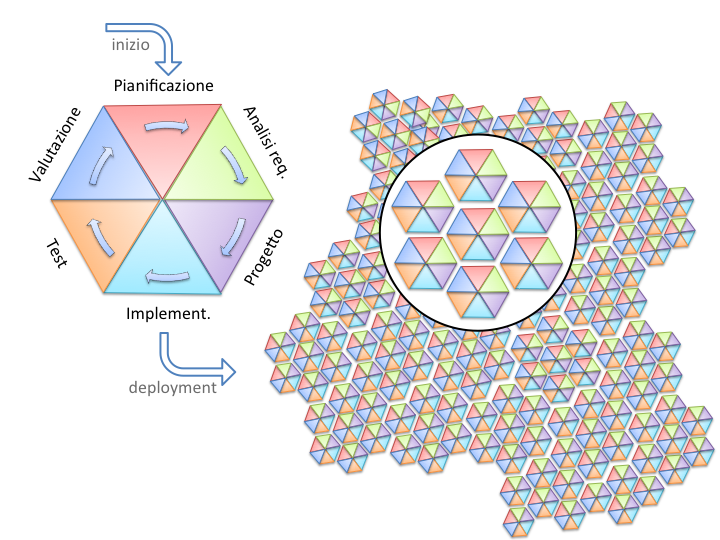
\includegraphics[scale=0.5]{img/modello_incrementale.png}
		\caption{Rappresentazione del modello incrementale\protect\footnotemark}
		\label{fig:modello_incrementale}
	\end{figure}

	\footnotetext{Fonte in \S\ref{rifinfo}}
	
	\section{Butterfly - C1} \label{c1}
    \subsection{Descrizione generale}
    Il capitolato C1 prevede lo sviluppo di Butterfly, un applicativo di supporto alle figure coinvolte nella produzione di un prodotto software che utilizzano strumenti con interfacce individuali che non sono in grado di comunicare fra di loro.
    Questo \gloss{progetto} è stato pensato viste le necessità di raggruppare queste notifiche e di fornire degli standard per interfacciarcisi oltre a permetterne una gestione automatizzata e personalizzabile per chi lo usa.

    \subsection{Obiettivo finale}
    Butterfly si presenta come un insieme di componenti che si interfacciano con gli strumenti di sviluppo in modo da recuperare o intercettare le segnalazioni che questi mandano e riportarle all'utente nella forma che quest'ultimo sceglie.\\
    Quest'applicativo deve essere in grado di incanalare le notifiche (contraddistinte da topic in base alla loro provenienza) di questi strumenti in un singolo broker che ne contolla l'inoltro verso un gestore%
    \footnote{Applicazione web richiesta dall'azienda che si interfaccia con Butterfly} interno all'azienda oppure direttamente alla persona interessata tramite applicazioni di messaggistica
    o email in base al topic con cui sono queste notifiche contrassegnate.

    \subsection{Tecnologie coinvolte}
    Si richiede l'utilizzo di un pattern \gloss{Publisher/Subscriber} per la gestione dei messaggi:

    \begin{itemize}
        \item \gloss{Producers}:
        \begin{itemize}
            \item \gloss{Redmine}
            \item \gloss{GitLab}
            \item \gloss{SonarQube}
        \end{itemize}
        \item \gloss{Broker}:
        \begin{itemize}
            \item \gloss{Apache Kafka}
        \end{itemize}
        \item \gloss{Consumers}:
        \begin{itemize}
            \item \gloss{Telegram}
            \item \gloss{Slack}
            \item \gloss{E-mail}
        \end{itemize}
    \end{itemize}
    I linguaggi indicati nel capitolato in cui l'applicativo può essere sviluppato sono: \gloss{Java}, \gloss{Python}, \gloss{Nodejs}.\\
    Sono inoltre richeste:
    \begin{itemize}
        \item \gloss{API REST} per interfacciarsi con i componenti dell'applicativo
        \item \gloss{Dockerfile} contenente le configurazioni necessarie per il container sul quale si andrà ad eseguire l'applicativo
        \item \gloss{The Twelve-Factor App} ovvero 12 fattori che le applicazioni sviluppate devono rispettare
    \end{itemize}

    \subsection{Valutazione conclusiva}
    La scelta di sviluppare il progetto presentato in questo capitolato permette al team di lavorare con un ampio ventaglio di tecnologie
    richieste sul mercato come \gloss{Docker} e Apache Kafka e questo ha motivato il gruppo a prenderne parte.\par
    Ha colpito molto la possibilità di creare un prodotto concreto e impiegato giornalmente dai developer che possa facilitarne il lavoro
    e automatizzare una parte del processo di sviluppo.\par
    Ha inoltre attirato l'attenzione del gruppo la consegna chiara e i vincoli precisi posti dall'azienda.\par
    D'altra parte l'impiego di numerose tecnologie richiede un impegno non indifferente e potrebbe risultare complesso.

	\section{Colletta - C2} \label{c2}
    \subsection{Descrizione generale}
    Il progetto \textit{Colletta} proposto dall'azienda Mivoq prevede la realizzazione di una piattaforma di collezione dati contenente piccoli esercizi di grammatica.
    In essa si identificano tre attori principali: insegnanti, allievi e sviluppatori. L'insegnante fornisce gli esercizi di grammatica che vengono svolti dagli allievi.
    I dati derivanti da queste interazioni tra insegnati e allievi possono in seguito essere utilizzate dagli sviluppatori per migliorare il sistema di riconoscimento delle frasi.

    \subsection{Obiettivo finale}
    L'obiettivo del progetto è creare un'applicazione (Web o mobile) con una struttura come quella descritta precedentemente,
    in cui la raccolta dei dati avviene in modo implicito tramite il solo utilizzo da parte degli utenti. Questi dati possono essere impiegati successivamente per la produzione di
    servizi utili basati sull'apprendimento automatico.

    \subsection{Tecnologie coinvolte}
    La scelta delle tecnologie viene lasciata libera, ma vengono consigliate:
        \begin{itemize}
            \item \gloss{Firebase} o altri servizi esistenti per l'immagazzinamento dei dati
            \item Software open-source per lo svolgimento degli esercizi:
            \begin{itemize}
                \item \gloss{Hunpos} 
                \item \gloss{Freeling}.
            \end{itemize}
        \end{itemize}

    \subsection{Valutazione conclusiva}
    Il capitolato appena descritto non è stato scelto da \gruppo\ perché tocca solo marginalmente l'ambito del \gloss{machine learning}.
    Tratta solamente di una piattaforma per la raccolta dati, motivo per cui non risulta particolarmente accattivante.
    La mancanza di vincoli non dà un'idea precisa di come sarebbe possibile operare per sviluppare il progetto.

    % TODO: machine learning da glossarizzare

	\section{G\&B - C3} \label{c3}
    \subsection{Descrizione generale}
    Il capitolato C3 parte dall'esigenza di dover monitorare i sistemi che nel prossimo futuro di occuperanno della fatture emesse in formato digitale. Data la grande mole di dati emessi, tali sistemi devono essere soggetti ad un continuo controllo. Per fare ciò si ricerca una stretta collaborazione tra "Development" e "Operation", detta anche "DevOps", grazie ad un efficiente sistema di notifica di eventuali problemi nei sistemi utilizzati.

    \subsection{Obiettivo finale}
    L'azienda proponente, come strumento di monitoraggio per questo tipo di sistemi, si affida a Grafana. Purtroppo Grafana si limita a segnalare eventuali problematiche principalmente nel momento in cui i parametri osservati superano un valore soglia. L'azienda vorrebbe dunque creare un plug-in per Grafana che sfrutti l'intelligenza artificiale attraverso una rete Bayesiana affinché il monitoraggio sia più efficace.

    \subsection{Tecnologie coinvolte}
    L'azienda consiglia / richiede di utilizzare:
    \begin{itemize}
    	\item \textbf{JavaScript}
    	\item \textbf{Grafana}
    	\item \textbf{Rete Bayesiana}: attraverso la libreria "jsbayes".
    	\item \textbf{GitHub}
    \end{itemize}

    \subsection{Valutazione conclusiva}
    Il capitolato richiede lo studio di strumenti inerenti l'intelligenza artificiale, un argomento ritenuto molto interessante dal gruppo. Purtroppo il dover creare un plug-in per un software già ben strutturato, quale Grafana, ha spinto il team a pensare che le tecnologie utilizzate fossero toccate in modo marginale.

	\section{MegAlexa - C4} \label{c4}

    \subsection{Descrizione generale}
    Il capitolato propone lo sviluppo di una piattaforma
    dedita alla creazione di una \gloss{routine} in grado di eseguire una sequenza
    di skill per Alexa, l'assistente vocale di \gloss{Amazon}.

    \subsection{Obiettivo finale}
    Nello specifico, \`e richiesto lo sviluppo di una piattaforma multilingua Web e
    mobile (\gloss{iOS} o \gloss{Android}) che sia in grado di
    creare \gloss{workflow} personalizzati per Alexa creati dagli utenti. Ogni utente
    deve aver la possibilit\`a di poter nominare i propri workflow senza collidere con
    quelli di altri utenti (e.g. un workflow chiamato "Buongiorno" dell'utente A \`e
    diverso dal workflow "Buongiorno" dell'utente B).

    \subsection{Tecnologie coinvolte}
    L'azienda consiglia di utilizzare:
    \begin{itemize}
    	\item Linguaggi per la piattaforma Web:
    	\begin{itemize}
            \item \gloss{HTML5}, \gloss{CSS3} (\gloss{Bootstrap}), Javscript
                per il \gloss{frontend}
            \item Node.js per il \gloss{backend}.
    	\end{itemize}
        \item \gloss{Kotlin}/\gloss{Swift}: linguaggi per lo sviluppo delle app
            rispettivamente per Android e iOS
        \item \gloss{Amazon Web Services} (AWS): servizio scelto per l'hosting del software e del database.
            Nello specifico, saranno utilizzati:
            \begin{itemize}
                \item \gloss{Amazon API Gateway}
                \item \gloss{AWS Lambda}
                \item \gloss{Amazon Aurora Serverless}
            \end{itemize}
    \end{itemize}

    \subsection{Valutazione conclusiva}
    Dall'analisi fatta dal team è stato deciso di non sviluppare questo capitolato per l'elevata mole di lavoro prevista.
    Non è semplice inoltre gestire le varie routine per gli utenti oltre che sviluppare un'applicazione Web e mobile nativa multilingua.
    Nonostante questo le tecnologie di AWS e di workflow di assistenti vocali risultano interessanti.

	\section{P2PCS - C5} \label{c5}
    \subsection{Descrizione generale}
    Il quinto capitolato propone la creazione di un'applicazione \gloss{Android} in grado di gestire una piattaforma di \gloss{car sharing}
    \gloss{peer to peer}.

    \subsection{Obiettivo finale}
    \`E richiesto lo sviluppo di un sistema software che consenta ad un utente la condivisione della propria auto. Tale condivisione si potrà
    avere solo una volta che l'operatore avrà inserito nel calendario i giorni in cui non utilizzerà il mezzo.
    In questo modo si lascia così la possibilità di poter dare le chiavi della propria autovettura in mano ad un'altro utente del servizio.

    \subsection{Tecnologie coinvolte}
    L'azienda consiglia di utilizzare:
        \begin{itemize}
        \item \gloss{Google Maps}
        \item \gloss{Google Cloud Platform}
        \item \gloss{Henshin - movens platform}
        \item \gloss{Octalysis}
        \item \gloss{Nodejs}
    \end{itemize}

    \subsection{Valutazione conclusiva}
    Fin da subito, l'idea di ``condividere la propria macchina con altre persone amiche o meno'' (cit. da capitolato) non ha suscitato interesse
    e motivazione al team. Inoltre, la tecnologia \textit{Octalysis} sembra vincolare troppo l'andamento del progetto: ne viene richiesto un
    uso stringente. Il risultato è un'applicazione che, secondo il parere del team di sviluppo, sfrutta il \gloss{gamification} per convincere gli utenti.
    Dopo queste considerazioni il team ha deciso di spostare i propri interessi verso altri capitolati.

	\section{Soldino - C6} \label{c6}
    \subsection{Descrizione generale}
    Redbabel Studio propone lo sviluppo di un sistema che consenta l'amministrazione delle \gloss{V.A.T.} imposte su beni venduti tramite \gloss{e-commerce}.
    \subsection{Obiettivo finale}

    L'obiettivo è quello di ottenere un prodotto che coinvolga l'intera gestione delle tasse, dal pagamento effettuato dal cliente per il singolo bene
    fino alla ricezione e gestione da parte del governo, passando per la ricezione della tassa da parte del \gloss{fornitore}.
    L'applicativo è composto da una parte che si occupa di gestire gli \gloss{smart contracts} e da una parte Web che permetta l'accesso alla \gloss{EVM}.

    \subsection{Tecnologie coinvolte}
	L'azienda consiglia:
    	\begin{itemize}
        \item \gloss{Ethereum}
		\item \gloss{Blockchain}
        \item Smart Contracts
		\item \gloss{EIP712}
		\item \gloss{Gas}
		\item \gloss{ERC20}
		\item \gloss{Reti Ethereum}
        \item \gloss{Reti Raiden}
        \item \gloss{Javascript ES8}
        \item \gloss{React/Redux}
        \item \gloss{SCSS}.
	\end{itemize}

    \subsection{Valutazione conclusiva}
    Nonostante l'uso di tecnologie innovative come Blockchain, smart contracts e gestione delle tasse in modo automatico, \gruppo\ non ha scelto
    il progetto perché richiede molto tempo da dedicare allo studio approfondito di tutti gli argomenti coinvolti.
    Essendo queste tecnologie nuove il team era indeciso se scegliere questo capitolato o optare su strumenti più consolidati.

\end{document}